\section{RS-232}

\subsection{Protocol}

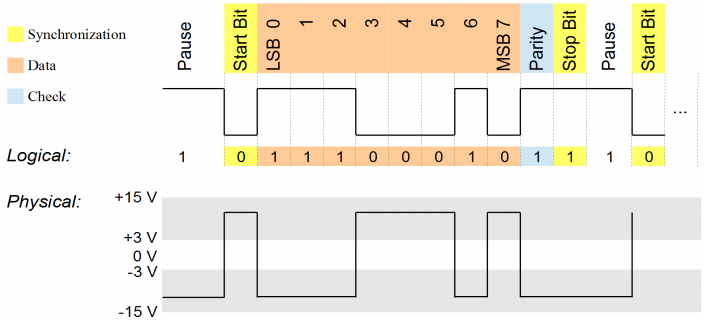
\includegraphics[width=0.5\textwidth]{rs232-protocol.png}

\begin{tabular}{lp{0.3\textwidth}}
    9600 8-O-1 & 9600 Baud, 8 Data Bits, Odd Parity, 1 Stop Bit \\
    Data Bits & 0100 0111 = 0x47 = 'G' \\
\end{tabular}

\begin{itemize}
    \item{
        \textit{
            RS-232 works with an \textbf{asynchronous} point to point transmission with
            seperate \textbf{Rx} and \textbf{Tx} data wires (Receive/Transmit).
        }
    }
    \item{
        \textit{
            Today more modern standards are used for the physical transmission
            of RS-232, e.g. USB or Bluetooth.
        }
    }
    \item{
        \textit{
            In practice \textbf{most often the parity-bit} is \textbf{not} used, but instead a check
            is done on a higher protocol layer, e.g. \textbf{CRC}-check sum.
        }
    }
\end{itemize}

\subsection{Transmission-protocols comparision}

\textit{
    Following protocols are used often with MCUs for wirebound transmission.
    (SPI «Serial Peripheral Interface» from Motorola, similar to Micro-wire of NI)
}

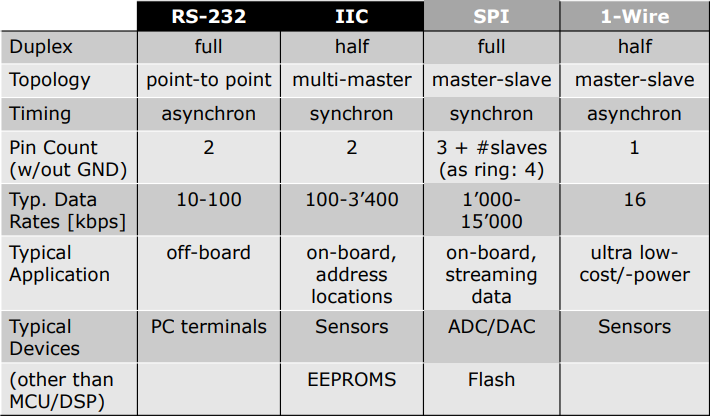
\includegraphics[width=0.5\textwidth]{transmission-protocols-overview.png}

\subsection{Function Schema \& Control Register}

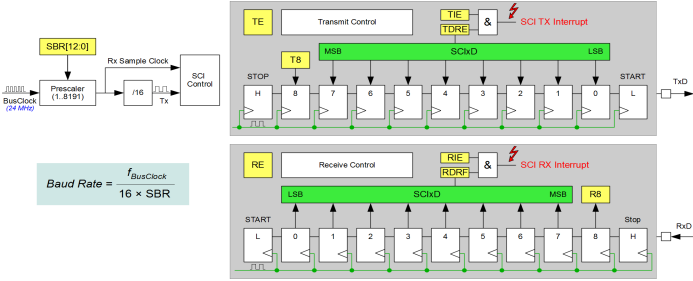
\includegraphics[width=0.5\textwidth]{rs232-schema.png}

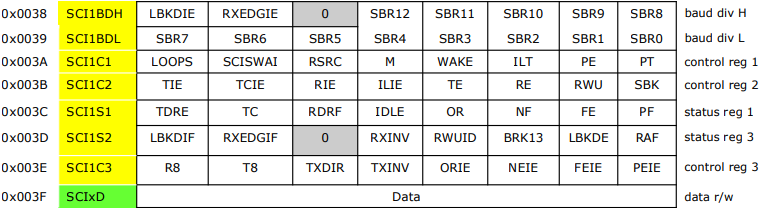
\includegraphics[width=0.5\textwidth]{rs232-control-register.png}

\subsection{Serial Bit-Synchronization}

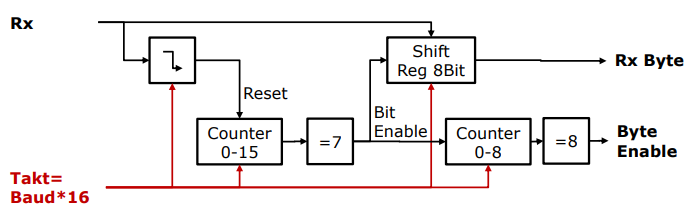
\includegraphics[width=0.5\textwidth]{rs232-serial-bit-synchronisation.png}

\begin{itemize}
    \item{\textit{
        Bit-Enable is the recovered bit clock rougly in the middle of each bit.
    }}
    \item{\textit{
        Serial transmitting fast fiber optical systems (eg. SDH) need a similar bit
        clock recovery (mostly done with Phase Locked Loops - PLL).
    }}
    \item{\textit{
        Missing parts: Byte-Enable should stop Counter0-15 - Reset should start it;
        bit sample eg. at positions 5, 7, and 9 – majority decision, 8-bit parallel
        load byte register, Tx.
    }}
    \item{\textit{
        noise bit is set if the 3 bits (5, 7 and 9) are not the same.
    }}
\end{itemize}

\subsection{Parity Bit}

\textit{
    E: Even parity = even count num 1 => 0 uneven num 1 => 1
    \newline
    O: odd is other way around
}

\subsection{Code RS232 with Ringbuffer}

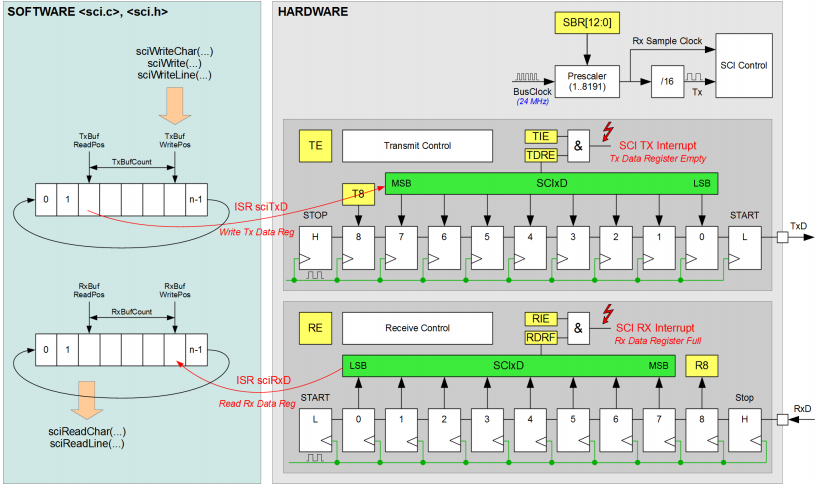
\includegraphics[width=0.5\textwidth]{rs232-ringbuffer.png}

\begin{lstlisting}
// sendqueue
static char tx1Buf[SCI1_TX_BUF_SIZE];
static uint8 tx1BufCount;
static uint8 tx1BufWritePos;
static uint8 tx1BufReadPos;

// receivequeue
static char rx1Buf[SCI1_RX_BUF_SIZE];
static uint8 rx1BufCount;
static uint8 rx1BufWritePos;
static uint8 rx1BufReadPos;

#define BUSCLOCK              24000000  // Hz

// init define baudrate; like 4800, 9600, 38400
void sci1Init(uint32 baudrate)
{
    // Berechnung Baudrate normalerweise: SCIxBD = Busclock / (16 x Baudrate)
    SCI1BD = (uint16) (((BUSCLOCK * (uint32) 10) / ((uint32) 16 * baudrate) + 5) / 10);

    SCI1C3 = 0x0F;              // activate error-Interrupts

    tx1BufCount = 0;            // TX-Buffer initialisieren
    tx1BufWritePos = 0;
    tx1BufReadPos = 0;

    SCI1C2_TE = 1;              // turn sender on

    rx1BufCount = 0;            // RX-Buffer initialisation
    rx1BufWritePos = 0;
    rx1BufReadPos = 0;

    SCI1C2_RE = 1;              // activate receiver;
    SCI1C2_RIE = 1;             // activate receiver interrupt
}

// error interrupt routine
interrupt void sci1Error(void)
{
    (void)SCI1S1;
    (void)SCI1D;
}

// receive data
interrupt void sc1RxD(void)
{
    char ch;
    (void)SCI1S1; // read state to reset
    ch = SCI1D;
    if(rx1BufCount < SCI1_RX_BUF_SIZE)
    {
        rx1Buf[rx1BufWritePos] = ch;
        rx1BufCount++;
        rx1BufWritePos++;
        if(rx1BufWritePos == SCI1_RX_BUF_SIZE) rx1BufWritePos = 0;
    }
}

// write next byte from ringbuffer
interrupt void sci1TxD()
{
    (void)SCI1S1;

    if(tx1BufCount != 0) {
        SCI1D = tx1Buf[tx1BufReadPos];
        tx1BufCount--;
        tx1BufReadPos++;
        if(tx1BufReadPos == SCI1_TX_BUF_SIZE) tx1BufReadPos = 0;
    } else {
        SCI1C2_TIE = 0;
    }
}

// write to the ringbuffer
char sci1ReadChar(void)
{
    char ch;
    while(rx1BufCount == 0);

    ch = rx1Buf[rx1BufReadPos];
    rx1BufCount--;
    rx1BufReadPos++;
    if (rx1BufReadPos == SCI1_RX_BUF_SIZE) rx1BufReadPos = 0;
    return ch;
}

// write a characater
void sci1WriteChar(char ch)
{
    while (tx1BufCount >= SCI1_TX_BUF_SIZE);

    tx1Buf[tx1BufWritePos] = ch;
    tx1BufCount++;
    tx1BufWritePos++;
    if (tx1BufWritePos == SCI1_TX_BUF_SIZE) tx1BufWritePos = 0;

    SCI1C2_TIE = 1;
}
\end{lstlisting}